\subsection{Modellagnostische Methoden - lokal}
\todo[inline]{Was noch fehlt: Für welche Art von Problemen funktionieren diese Algorithmen? LIME nur für Klassifikation, aber die anderen? Vor- und Nachteile ausbauen...}

Folgendes Unterkapitel fasst eine Auswahl an Methoden zusammen, welche als modellagnostisch und lokale Ansätze einzuordnen sind (für eine Erklärung der Begriffe siehe Kapitel \ref{subsubsec:Erklaeransaetze}). Alle diese Ansätze, da sie modellagnostisch sind, haben gemeinsam, dass keine Zugriff auf die Modellstruktur notwendig ist. Es muss lediglich möglich sein Vorhersagen für Dateninstanzen abrufen zu können.

\subsubsection{LIME}
\label{subsubse_LIME}
Die Methode \emph{LIME}, entwickelt von \textcite{ribeiro2016should}, wurde in der betrachteten Literatur am häufigsten genannt (sieht z.B.: \cite{weitz2019you}, \cite{goldenfein2019algorithmic}, \cite{tsiakmaki2021case}, \cite{tjoa2020survey}, \cite{hanif2021survey}, \cite{krause2017workflow}, \cite{gomez2021advice}, \cite{wang2020explainable}, \cite{strobel2019aspects}, \cite{westin2020building}, ...)
LIME steht für \emph{Local Interptetable Model Agnostic Eplanations} und erklärt einzelne Vorhersagen eines jeden Klassifikationsalgorithmus, indem ein interpretierbares Modell lokal um eine zu erklärende Instanz herum gelernt wird \cite{ribeiro2016should}. Diese Erklärtechnik wird als lokaler Stellvertreter (eng.: \emph{Local Surrogate}) bezeichnet \cite{molnar2022}. 

%Dieses Modell ist meistens ein lineares Modell, was um die einzelnen Instanzen gebaut wird, die erklärt werden sollen. 
\textbf{Konzept}

Bei LIME kommt es zu einer lokalen Annäherung an ein Black-Box-Modell ($f$) durch ein zu interpretierbares Modell ($g$). Nach \textcite{ribeiro2016should} setzt LIME daher eine Abwägung zwischen Genauigkeit und Interpretierbarkeit voraus. Beispiel für interpretierbare Modelle sind in Kapitel \ref{subsubsec_transparenteModelle}) zu sehen.
In Abbildung \ref{Fig:Lime-Funktionsweise} sind die zwei Modelle $f$ und $g$ sowie verschiedene Instanzen zu sehen. Die rosa und die blauen Flächen demonstrieren die Funktionsweise des Black-Box-Modells, welche komplex und nicht-linear ist. Ziel von LIME ist es nun, zu erklären, warum eine bestimmte Instanz (das große rote Kreuz in der Mitte der Abbildung) in die Klasse \enquote{rosa} einsortiert wurde. Die LIME-Methode konzentriert sich nun als lokaler Ansatz auf den Bereich, um diese zu erklärenden Instanz. Um die zu erklärende Instanz herum werden nun zufällig weitere Datenpunkte erzeugt (Pertubationen). Dies ist durch die blauen Punkte und roten Kreuze dargestellt. Für diese Pertubationen, wird nun die Zielvariable mithilfe des Black Je näher sich diese Pertubationen an der zur erklärenden Instanz befinden, desto stärker fallen sie ins Gewicht. Nun wird sich mithilfe eines interpretierbaren Modell $g$ an dieser Instanz dem Black-Box-Modell $f$ angenähert. $g$ kann nun von Menschen interpretiert werden \cite{ribeiro2016should}. In der Abbildung würde ein Mensch also sehen, dass alles Werte links der gestrichelten Linie der Klasse \enquote{rosa} zuzuordnen sind. Alle Werte rechts der Linie, würden als \enquote{blau} klassifiziert werden. Hier wird noch einmal deutlich, dass LIME lediglich lokale Erklärungen erzeugt, denn Instanzen, welche sich auf dem Bild ganz links, weit entfernt der Entscheidungslinie befinden, gehören der blauen Klasse an. So ist die lokale Erklärung hier richtig, aber lässt global falsche Schlüsse zu.
\begin{figure}
    \centering
    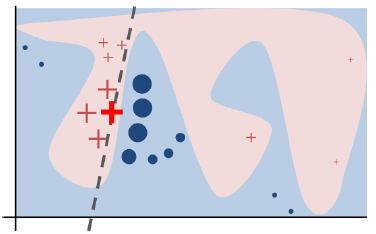
\includegraphics[scale=0.45]{pic/MA-Bilder/Literaturrecherche/LIME.PNG}
    \caption{Funktionsweise von LIME, entnommen aus: \cite{ribeiro2016should}}
    \label{Fig:Lime-Funktionsweise}
\end{figure}

\textbf{Formale Betrachtung}
Ziel von LIME ist das Finden des lokalen Stellvertreters, der lokal die eine bestimmte Instanz $x$ erklärt. Dieses Modell sollte so einfach wie möglich sein. Jedoch sind nicht alle Modelle gleich verständlich. So gibt es unterschiedliche Instanzen $g$ aus der Klasse $G$, die alle Instanzen von z.B. linearen Funktionen enthält. $G$ kann jedoch theoretisch auch die Menge aller Entscheidungsbäume sein \cite{ribeiro2016should}. So führen \textcite{ribeiro2016should} den Faktor  $\Omega(g)$ ein. Dieser misst die Komplexität eines interpretierbaren Modells, dies kann bei Entscheidungsbäumen beispielsweise die Tiefe eines Baums sein oder bei linearen Modellen die Anzahl an Gewichten. Nach \textcite{ribeiro2016should} kann nun eine Erklärung für den Datenpunkt $x$ durch folgendes Optimierungsproblem gefunden werden:
\begin{equation}
    \xi(x) = \underset{g \in G}{argmin} \mathcal{L}(f, g, \pi_{x}) + \Omega(g)
\end{equation}
$\mathcal{L}(f, g, \pi_{x})$ gibt an, dass eine gute Abschätzung an das Black-Box-Modell $f$ gefunden werden soll, welches sich in der Nachbarschaft $\pi_{x}$ befindet. Des Weiteren soll das gefundene Modell $g$ so einfach wie möglich sein, was durch $\Omega(g)$ angegeben ist \cite{ribeiro2016should}. Z.B. kann $\Omega(g)$ ausdrücken wie viele Merkmale von der interpretierbaren Funktion $g$ erfasst werden soll \cite{molnar2022}.
Um nun ein gutes Modell $g$ zu finden, muss der erste Therm der Formel optimiert werden. Hierfür wird sich die Nachbarschaft angesehen und dort lokal ein Modell gefunden. Ziel ist es das Modell mit der höchsten Genauigkeit zu finden. Dies geschicht, indem für alle Datenpunkte in der Nachbarschaft aus Abbildung \ref{Fig:Lime-Funktionsweise} sowohl das interpretierbare Modell $g$ als auch das Black-Box Modell $f$ aufgerufen wird. $g$ wird nun daraufhin optimiert, so wenig Fehler wie möglich zu haben, was mit den Vorhersagen des Black-Box-Modells überprüft werden kann. Bei diesem Optimierungsproblem fallen Punkte, die näher an $x$ liegen stärker ins Gewicht. 
%Diese Formel kann mit verschiedenen Erklärungen $G$, Funktionen $\mathcal{L}$ oder Komplexitätsmaßen $\Omega$ genutzt werden.

%So sind nicht alle interpretierbaren Modelle (vgl. Kapitel \ref{subsubsec_transparenteModelle}) im gleichen Maße für Menschen verständlich. \textcite{ribeiro2016should} definieren in ihrem Paper eine Erklärung als $g \in G$, wobei $G$ alle interpretierbaren Modelle (z.B. Entscheidungsbäume oder lineare Modelle) enthält. 
%Bevor eine Erklärung von LIME präsentiert wird, werden zunächst kurz Grundlagen bzgl. der Interpretierbarkeit von Modellen erläutert. Zuallererst ist es wichtig, sich den Unterschied zwischen Merkmalen, welche das Black-Box-Modell verwenden, und für Menschen interpretierbaren Daten zu verdeutlichen. \textcite{ribeiro2016should} demonstrieren dies mit einem Beispiel aus der Texklassifikation. Ein binärer Vektor, der beschreibt, ob sich ein bestimmtes Wort in einem Text befindet und somit zur Klassenvorhersage führte, ist für den Menschen interpretierbarer als die Datenstruktur, welche durch den Algorithmus in Wahrheit (z.B. Wordembeddings) zur Bearbeitung der Klassifikationsaufgabe genutzt wird. Formal definieren sie $ x \in \mathds{R}^{d}$ als originale Repräsentation, während $ x' \in \{0,1\}^{d'}$ die binäre Repräsentation ist, welche für Menschen interpretierbar ist. 

%\begin{figure}[h]
%    \centering
%    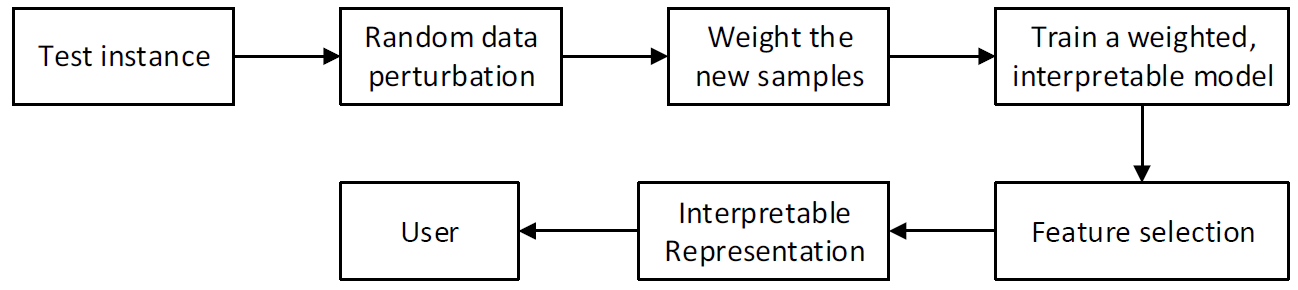
\includegraphics[scale=0.45]{pic/MA-Bilder/Literaturrecherche/LIME-Ablauf.PNG}
%    \caption{Ablauf von LIME, entnommen aus: \cite{zafar2019dlime}}
%    \label{Fig:Lime-Ablauf}
%\end{figure}

%\cite{kamath2021explainable}: der Verlust von $\mathcal{L}$ wird nun abgeschätzt, indem zufällige Pertubationen $z$ um die Instanz die erklärt werden soll erzeugt werden. Diese Datensätzen werden gewichtet mithilfe von $\pi_{x}(z)$, um die Distanz zu bestimmen.

\textbf{Anwendung von LIME}

Ein Beispiel für eine mit LIME erzuegte Erklärung ist in Abbildung \ref{Fig:Lime-Beispiel} dargestellt. Hier wurde anhand verschiedener Werte untersucht, ob eine Person Diabetes hat. Hier wurde eine Person mit einer Wahrscheinlichkeit von ungefähr 60 (links dargestellt) als Diabetes-Patient eingeordnet. Diese Entscheidung wird vor allem durch die orange dargestellten Merkmale unterstützt, so z.B. das Alter. Blau markiert sind solche Merkmale, welche eher für einen gesunden Patienten sprechen würden. Rechts sind zur Übersicht die Merkmalswerte aufgezeigt.
\begin{figure}
    \centering
    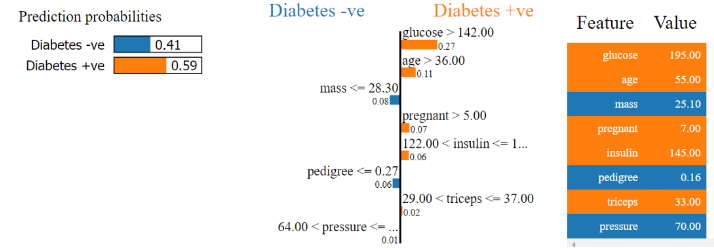
\includegraphics[scale=0.45]{pic/MA-Bilder/Literaturrecherche/LIME-Erklaerung-Beispiel.PNG}
    \caption{Erklärung der Klassifikation einer bestimmten Instanz, entnommen aus \cite{LIME-beispiel}}
    \label{Fig:Lime-Beispiel}
\end{figure}
Zur praktischen Umsetzung von LIME stellen die Erfinder eine Bibliothek\footnote{https://github.com/marcotcr/lime} zur Verfügung. LIME kann für jeden Klassifikationsalgorithmus auf tabellarischen Daten, Text oder auch Bilder angewendet werden. Weiter kann durch den Entwickler ausgewählt werden, wie viele Merkmale dargestellt werden sollen \cite{molnar2022}. Je nach dem, welche Daten dem Klassifikationsalgorithmus zu Grunde liegen, kommt es zu leichten Unterschieden in der Anwendung. So muss zwischen Merkmalen, mit denen ein Algorithmus arbeitet und Merkmalen, welche für Menschen interpretierbar sind, unterschieden werden \cite{ribeiro2016should}. \textcite{ribeiro2016should} demonstrieren dies mit einem Beispiel aus der Texklassifikation. Ein binärer Vektor, der beschreibt, ob sich ein bestimmtes Wort in einem Text befindet und somit zur Klassenvorhersage führte, ist für den Menschen interpretierbarer als die Datenstruktur, welche durch den Algorithmus in Wahrheit (z.B. Wordembeddings) zur Bearbeitung der Klassifikationsaufgabe genutzt wird \cite{ribeiro2016should}. Bei Textklassifikation werden nun Permutationen dadurch erzeugt, dass zufällig Wörter aus einem Text etfernt werden. Die Klasse wird danndamit erklärt, ob oder wie oft ein bestimmtes Wort in einem Text vorkam.

\textbf{Vor- und Nachteile}

Die Formel von LIME kann mit unterschiedlichen ML-Methoden von $f$ und $g$ genutzt werden \cite{ribeiro2016should}. Dies bedeutet, das zugrundeliegende Black-Box Modell kann ausgetauscht werden, während der lokale Stellvertreter $g$ nicht geändert werden muss. Auch kann ein lokaler Stellvertreter genutzt werden, welchen die Erklärungsbetrachter gut verstehen, weil schon Vorwissen vorhanden ist (z.B. Entscheidungsbäume) \cite{molnar2022}. 
\textcite{ribeiro2016should} stellen in ihrer Veröffentlichung besonders heraus, dass LIME Vertrauen in ML-Algorithmen erhöhen kann und zur Erkennung von unerwünschten Verhalten beiträgt. So weisen sie auf einen Klassifikationsalgorithmus hin, welcher Fotografien von Wölfen und Huskys unterscheiden sollte. LIME ermöglichte es, aufzudecken, dass dieser Algorithmus solche Bilder mit Schnee im Hintergrund, der Klasse Husky zuordnete und die Tiere selbst gar nicht beachtete \cite{ribeiro2016should}.

Nachteil ist die Schwierigkeit bei tabellarischen Daten, die Nachbarschaft zu bestimmen \cite{molnar2022}. Weiter entdeckten \textcite{slack2020fooling} eine Möglichkeit, dass sich Erklärungen manipulieren lassen um Bias in den Daten zu verstecken, was zu Vertauensverlust führen kann.  Daneben werden die Daten immer zufällig generiert, sodass gleiche Instanzen unterschiedliche Erklärungen erhalten können. Dieses Problem löst eine Abwandlung von LIME. \textcite{zafar2019dlime} entwickelten DLIME (\emph{Deterministic Local Interpretable Model-Agnostic Explanations Approach for Computer-Aided Diagnosis Systems}). Hier werden die Pertubationen anders generiert (agglomeratives hierarchisches Clutering) und für die Auswahl der sich der zur erklärenden Instanz am nächsten befindlichen Datenpunkte den in Kapitel \ref{subsubsec_KNN} beschriebenen KNN-Algorithmus nutzen.

\subsubsection{SHAP}
Auch die modellagnostische Methode \emph{SHAP} wurde von vielen Autoren genannt (\cite{tsiakmaki2021case}, \cite{vaughan2020human}, \cite{schoeffer2022human}, \cite{hanif2021survey}, \cite{gomez2021advice}, \cite{wang2020explainable}, \cite{palaniyappan2022aqx}, ...). Diese Methode wurde zuerst von \textcite{lundberg2017unified} vorgestellt und basiert auf den sogenannten SHAPLEY-Werten aus der Spieltheorie. SHAPLEY-Werte beantworten die Frage, was ein einzelner Spieler innerhalb einer Gruppe beitrug. Angewendet auf das Forschungsfeld des MLs können einzelne Spieler als Merkmalswerte betrachtet werden\cite{wang2020explainable}.

\textbf{Konzept}

Die Shapley-Werte wurden von \textcite{shapley1951notes} eingeführt. Gegeben ist eine Gruppe von Spieler, welche gemeinsam einen Wert $v$ erzielen. In dem Beispiel von \textcite{molnar2022} ist dies ein Preis für eine Wohnung. Verschiedene Spieler oder im ML-Kontext Merkmale wirken sich unterschiedliche auf einen Wohnungspreis aus. Beispielhafte Merkmale können hier das Stockwerk, die Lage oder das Verbot von Haustieren sein. Um nun den Beitrag eines Merkmals zu berechnen, kann nun getestet werden, welchen Wohnungspreis ohne ein bestimmtes Merkmal erzielt werden würde. Nun wird dieses Merkmal, z.B. das Haustierverbot, ausgeklammert und der Wohnungspreis berechnet. Dies muss für alle Kombinationen, wo das Haustierverbot fehlt, geschehen, um Abhängigkeiten zwischen Merkmalen zu erkennen. Nun wird die Differnez zwischen dem ursprünglichen Wert $V$ und dem neuen Ergebnis berechnet. Über alle Ergebnisse wird der Durchschnitt gebildet. Dies geschieht für alle anderen Merkmale analog. Somit erhält man die Shapley-Werte für alle Merkmale \cite{molnar2022}.

\textbf{Formale Betrachtung}
textcite{lundberg2017unified} wenden dieses Konzept in ihrer Methode (SHAP (\emph{SHAPLEY ADDITIVE EXPLANATIONS})) an, um einzelne Vorhersagen zu erklären, indem Beiträge eines jeden Merkmals berechnet werden. Sei $x$ die zu erklärende Instanz und $f(x)$ das Black-Box-Modell. Zu $x$ existieren noch vereinfachte lokale Eingabe $x'$. Dieses muss eingeführt werden, um die Werte der Merkmale zu vereinfachen, so werden sie z.B. als binäre Vektoren dargestellt. Weiter existiert für das Black-Box-Modell ein Modell $g$, für das gilt $g(x') \approx f(x)$. $g$ sieht weiter wie folgt aus und gibt an, was ein Merkmal zu einer Vorhersage einer Instanz $x'$ beiträgt (vereinfacht von \cite{Gianfagna.2021} nach \cite{lundberg2017unified}):
\begin{equation}
    g(x') = \phi_{0} + \sum\limits_{i=1}^{M}\phi_{i}x'_{i}
\end{equation}
Mit $\phi_{0}$ ist der sogenannte \emph{Null-Output} und meint den durchschnittlichen Output des Modells, den von den einzelnen Merkmalen unabhängig ist. $i$ ist ein Merkmal und $M$ ist die Anzahl aller Merkmale. $\phi_{i}$ ist der Erklärungseffekt eines Merkmals $i$ und gibt an, wie viel dieses Merkmal zu einer Veränderung der Vorhersage beiträgt \cite{lundberg2017unified}. 


\textbf{Anwendung}
\textcite{lundberg2017unified} stellen eine Bibliothek\footnote{https://shap.readthedocs.io/en/latest/index.html} für die Nutzung von SHAP zur Verfügung. Dort ist auch aufgelistet, worfür SHAP verwendet werden kann, z.B. für Klassifikation oder Regression. Ein Beispiel für eine mit SHAP generierte Erklärung ist in Abbildung \ref{Fig:Beispiel_Shap} dargestellt. Hier wird die Ausgabe des Wertes 0,4, welche durch ein Black-Box-Modell erstellt wurde, erklärt. Merkmale, welche die Vorhersage in einen höheren Wert ändern, wie z.B. das Alter, sind rot eingezeichnet. Blau eingezeichnete Merkmale, wie z.B. das Geschlecht würden den Wert der Vorhersage verringern.
\begin{figure}
    \centering
    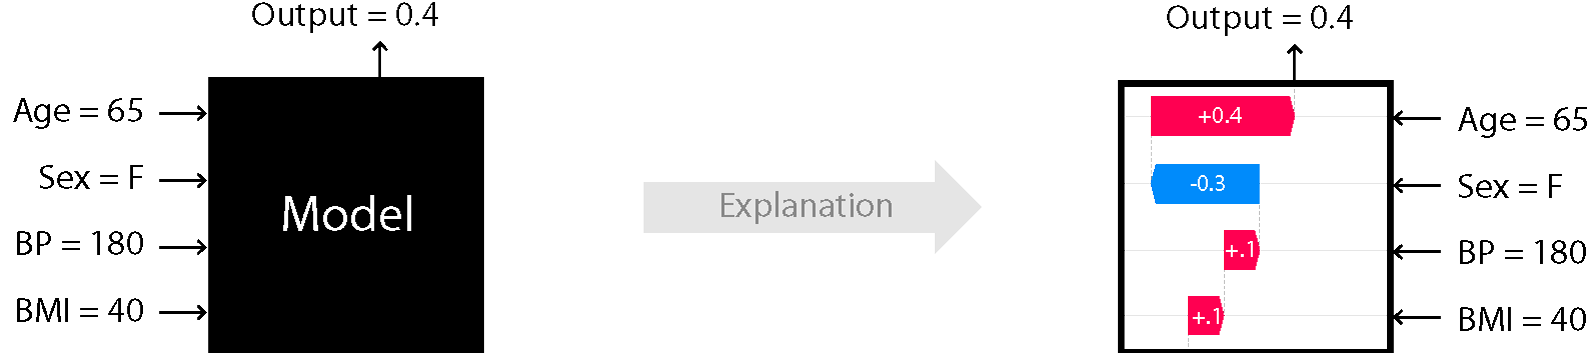
\includegraphics[scale=0.45]{pic/MA-Bilder/Literaturrecherche/SHAP-Beispiel.PNG}
    \caption{Beispiele Erklärungen mit SHAP, entnommen aus der SHAP Bibliothek}
    \label{Fig:Beispiel_Shap}
\end{figure}
Ein praktisches Problem mit SHAP besteht in der Berechnung der SHAPLEY-Werte. Würden 4 Features vorliegen, müssen 16 verschiedene Möglichkeiten für die Exkludierungen der Features berechnet werden. Bei 32 Features, wären dies schon 17,1 Milliarde Berechnungen. Hierfür haben \textcite{lundberg2017unified} den Shapley Kernel entwickelt, welcher sich SHAPLEY-Werte annähert und weniger Datensätze erstellen muss. Für Kernel SHAP definieren die Autoren auch Sonderformen, wie z.B. Deep SHAP für DL, welche sich die Funktionsweise der zugrunde liegenden ML-Modelle zunutze machen.
SHAP kann weiterhin auch für globale Erklärungen verwendet werden, wenn diese für jede Instanz angewendet wird \cite{molnar2022}.

\textbf{Vor- und Nachteile}
Nach \textcite{lundberg2017unified} grenzen sich SHAP-Erklärungen von anderen Erkläransätzen ab, da sie drei wichtige Eigenschaften erfüllen: lokale Genauigkeit, Fehlen, Konsistenz.
Als erste wünschenswerte Eigenschaften wird lokale Genauigkeit definiert, so muss das Erklärungsmodell $g$ das Black-Box-Modell $f$ approximieren, sodass auch die Ausgaben von $f$ und $g$ ungefähr übereinstimmen. Des Weiteren sollten auch die Werte der Erklärungen 0 für nicht vom Modell betrachtete Features sein (Eigenschaft: Fehlen). Die dritte Eigenschaft ist Konsistenz \cite{lundberg2017unified}. So sollte eine Zunahme (oder Gleichbleiben) eines Merkmalswertes bedingen, dass auch der SHAPLEY-Wert zunimmt (oder gleich bleibt). Weiter basiert SHAP auf einer soliden wissenschaftlichen Grunglage und beziehen bei ihrer Erklärung alle Merkmale mit ein. Laut \textcite{molnar2022} macht sie dies zu einer geeigneten Methode, das Recht auf Erklärungen der DSGVO umzusetzen. Daneben können sowohl lokale als auch globale Erklärungen generiert werden \cite{molnar2022}. Ein Nachteil dieser Methode besteht jedoch auch in den Shapley-Werten an sich. Da sie immer jedes Merkmal beachten, sind Shapley Werte, die falsche Wahl, wenn dem Nutzer nur einige wenige Merkmale präsentiert werden sollen. Hier sei LIME besser geeignet, da hier die Reduktion auf einige wenige Merkmale möglich ist.
Ein weiterer Nachteil, der jedoch auch für LIME gilt, sit die von \textcite{slack2020fooling} entdeckte Manipulationstechnik, welche angewendet werden kann, um Bias in den Daten zu verstecken. Weiter ist auch die Berechnung mit dem SHAP-Kernel recht langsam und aufwendig \cite{molnar2022}.

\subsubsection{Anchors}
Die folgende Methode wurde von den selben Wissenschaftlern entwickelt, welche auch LIME vorgestellt hatten und produziert Wenn-Dann-Regeln, die \enquote{Anchors} genannt werden \cite{ribeiro2018anchors}.

\textbf{Konzept}
Der folgende Ansatz setzt auf einer Schwäche der LIME-Methode auf. Wie in \ref{subsubse_LIME} beschrieben, werden Erklärungen mittels LIME durch lokale Annäherungen an bestimmte Instanzen produziert. In der Abbildung \ref{Fig:Lime-Funktionsweise} wurde gezeigt, dass alles lokal links der Entscheidungslinie der rosa Klasse zuzuordnen war, wenngleich sich links, weiter entfernt der Entscheidungslinie Instanzen befanden, welche als blau zu klassifizieren sind. LIME beantwortet also nicht die Frage, für welche Instanzen ihre Erklärung übertragbar ist. Dieses Problem wird von \textcite{ribeiro2018anchors} allerdings mit Hilfe der Anchors adressiert.
In Abbildung \ref{Fig:Funktionsweise_Anchors} sind die Funktionsweise von LIME und Anchors zusammen dargestellt. Die jeweiligen Kästchen stellen die Wenn-Dann-Regeln dar. Diese bringen ihre Grenzen zum Ausdruck und geben genau an, für welche Umgebung sie gültig sind.
\begin{figure}
    \centering
    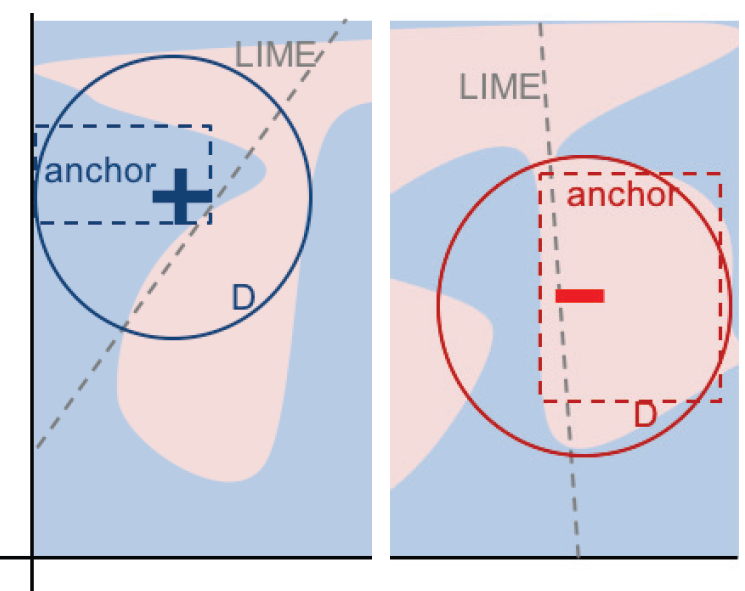
\includegraphics[scale=0.45]{pic/MA-Bilder/Literaturrecherche/Anchor.PNG}
    \caption{Funktionsweise der Anchors, entnommen aus \cite{ribeiro2018anchors}}
    \label{Fig:Funktionsweise_Anchors}
\end{figure}


%\begin{figure}[h]
%    \centering
%    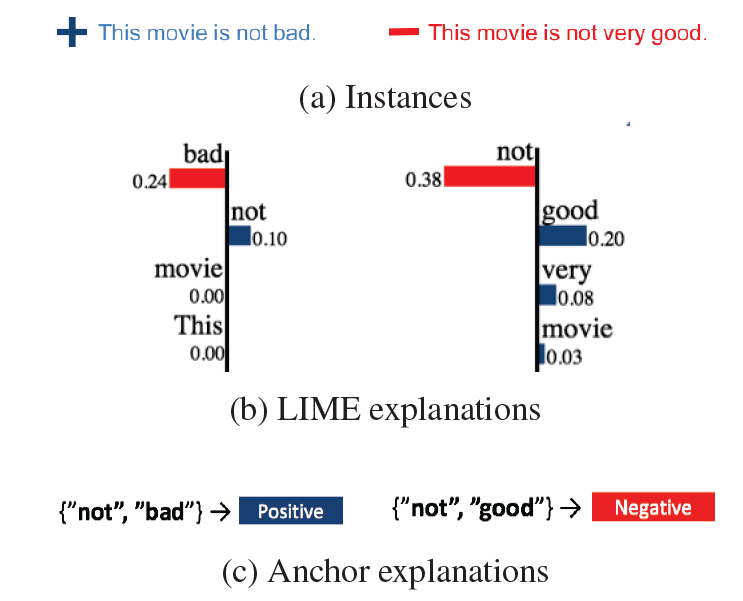
\includegraphics[scale=0.45]{pic/MA-Bilder/Literaturrecherche/Anchors-Probleme-mit-LIME.PNG}
%    \caption{Erklärungen LIME vs. Anchors, entnommen aus: \cite{ribeiro2018anchors}}
%    \label{Fig:Probleme_LIME}
%\end{figure}
%Diese Methode sollte auch eine Schwäche von LIME abdecken, welche in der Coverage (dt.: Abdeckung) besteht. Wie in \ref{subsubse_LIME} beschrieben, werden Erklärungen mittels LIME durch lokale Annäherungen an bestimmte Instanzen produziert. Was jedoch offen bleibt, ist die Frage, ob sich solche Erklärungen auch auf andere Datenpunkte übertragen lassen. Für die Nutzer eines Systems kann dies jedoch wichtig sein, um die Funktionsweise eines Systems zu verstehen und den Erklärungen vertrauen zu können, wenn genau festgelegt ist, für welche Instanzen eine Erklärung anzuwenden ist \cite{ribeiro2018anchors}. Illustriert wird dieses Problem von den Autoren selbst. So wurden sowohl mittels LIME als auch mittels Anchors Erklärungen für einen Textklassifikationsalgorithmus erstellt. Das Wort \enquote{not} ist für zwei unterschiedliche Klassenvorhersagen wichtig gewesen. Probleme können passieren, wenn Nutzer eines Systems, die Erklärung, welche mittels LIME für den Satz \enquote{The movie is not very good} auf den Satz \enquote{The movie is not bad} anwenden. Um Missverständnisse auf Nutzerseite zu vermeiden ist es wichtig, mehrere Gründe mitzugeben, die erklären, warum ein Satz welcher das Wort \enquote{not} enthält, als positiv klassifiziert wurde.

 %(\ref{Fig:Probleme_LIME}) 
 
\textbf{Formale Betrachtung}
Sei nach \textcite{ribeiro2018anchors} $f$ das Black-Box-Modell und $x$ die zu erklärende Instanz. Weiter kommt es zu einer Pertubation um $x$ herum, dessen Verteilung als $D$ definiert ist. Um einen Anchor zu definieren sei nun $A$ eine Regel, die aus einer Menge von Aussagen besteht. $A(x)$ ist dann 1, wenn alle Merkmalsaussagen wahr sind, für eine Instanz $x$. In einem Textklassifikationbeispiel, was z.B. den Satz \enquote{The Movie is not bad} als positive Aussage klassifiziert ist, $X$ der Satz und $f(x)$ positiv. Weiter wäre hier die Regel $A=\{ not, bad \}$. In Worten könnte die Regel wie folgt formuliert werden: \emph{Wenn die Wörter not und bad vorkommen, ist die Klasse positiv.} 
Sei nun $D(\cdot{}|A)$ die Verteilung von Instanzen, auf die $A$ auch zutrifft (z. B. ähnliche Texte, in denen \enquote{not} und \enquote{bad} vorkommt) \cite{ribeiro2018anchors}. $\mathcal{T}$ auf der rechten Seite der Formel gibt eine Präzisionsschwelle an. So sollen nur solche Wenn-Dann-Regeln als gültig erachtet werden, wenn sie eine lokale Treue von mindestens $\mathcal{T}$ erreichen. Formal sei also ein Anchor definiert als \cite{ribeiro2018anchors}:
\begin{equation}
    \mathds{E}_{D_{(z|A)}}[\mathbb{1}_{f(x)=f(z)}]\geq \mathcal{T}, A(x)=1
\end{equation}
\textcite{molnar2022} gibt diese Formel in eigenen Worten wieder: Wenn eine Instanz $x$ erklärt werden soll, kann dies mit einem Anchor geschehen, welcher für $x$ gilt. Hierbei sollte, die selbe Klasse für die Nachbarn von $x$ mit einer Wahrscheinlichkeit von $\mathcal{T}$ vorausgesagt werden, damit dieser Anchor anwendbar bleibt. Die Genauigkeit einer Regel ergibt sich durch das Aufrufen des Black-Box-Modells für die Nachbarn, hier notiert mit $[\mathbb{1}_{f(x)=f(z)}]$.

\textbf{Anwendung}
\textcite{ribeiro2018anchors} zeigen in ihrer Veröffentlichung die Anwendung von Anchors für Klassifikation, strukturierte Vorhersagen und Textgenerierung auf Grundlage verschiedener Datentypen (tabellarisch, textuell, visuell). Auch für das Erstellen von Anchors gibt es eine Bibliothek\footnote{https://github.com/marcotcr/anchor}, welche Entwickler unterstützt.
Für das Finden von Anchors existieren mehrere Ansätze. Ein einfacher \enquote{Bottom-Up-Ansatz} beruht darauf, mit einer leeren Regel zu starten und in Iterationen dieser Regel einen neuen Merkmalswert hinzuzufügen. Getestet würde diese Regel dann mit einer Prüfung der Genauigkeit $\mathbb{1}_{f(x)=f(z)}$  für jeden Nachbarn von $x$ \cite{ribeiro2018anchors}. Dies wäre jedoch in bei der Arbeit mit großen Datensätzen oder mit sehr vielen Merkmalsvariablen zu rechenaufwendig \cite{molnar2022}.
Daher schlagen die Autoren vor lediglich Stichproben zu ziehen und auf statistisches Vertrauen in die Genauigkeit zu setzen. Technisch geschieht die Suche, welche auch in der Anchors-Bibliothek implementiert ist mit einem Reinforcement-Learning-Ansatz (Multi-Armed-Bandit), welcher für die Modellaufrufe zuständig ist, die für das Evaluieren von Regeln sorgen. Um die besten Kandidaten für eine mögliche Wenn-Dann-Regel $A$ in die nächste Runde zu übertragen wird wird eine Balkensuche (modified Beam Search) angewendet \cite{ribeiro2018anchors}. Wie viele Kandidaten durch diese Suche begutachtet werden, bestimmt auch die geforderte Rechenleistung und die zu erreichende Genauigkeit \cite{molnar2022}
%Daher schlagen die Autoren vor den Parameter $\delta$ vor, welcher zwischen 1 und 0 liegen sollte, um eine probabilistische Definition zu erstellen. Hierdurch werden so lange Stichproben gezogen, bis statistisches Vertrauen in ihre Genauigkeit besteht. Die probabilistische Definition lautet wie folgt \cite{ribeiro2018anchors}:
%\begin{equation}
%    P(prec(A) \geq \mathcal{T}) \geq 1 - \delta  
%\end{equation}
%wobei gilt:
%\begin{equation}
%    prec(A) = \mathds{E}_{D_{(z|A)}}[\mathbb{1}_{f(x)=f(z)}]
%\end{equation}
%Weiter ist es das Ziel, die Abdeckung $cov(A) = \mathds{E}_{D_{(z|A)}}[A(z)]$ zu maximieren, also den Bereich, in der ein Anchor anzuwenden ist. Dies ist in sofern sinnvoll, als dass Regeln mit höherer Abdeckung stärker ins Gewicht fallen, da sie einen größeren Teil des Modells beschreiben. Auf der anderen Seite, sind Regeln mit einer geringeren Abdeckung präziser, sodass hier eine Abwägung zwischen Genauigkeit und Abdeckung sattfinden muss.

%Abbildung \ref{Fig:Anchors_Finden} \todo{diese Abbildung kommt wahrscheinlich noch in den Anhang} gibt einen kurzen Überblick bzgl. des Entstehungsprozesses von Anchors: 
%\begin{figure}
%    \centering
%    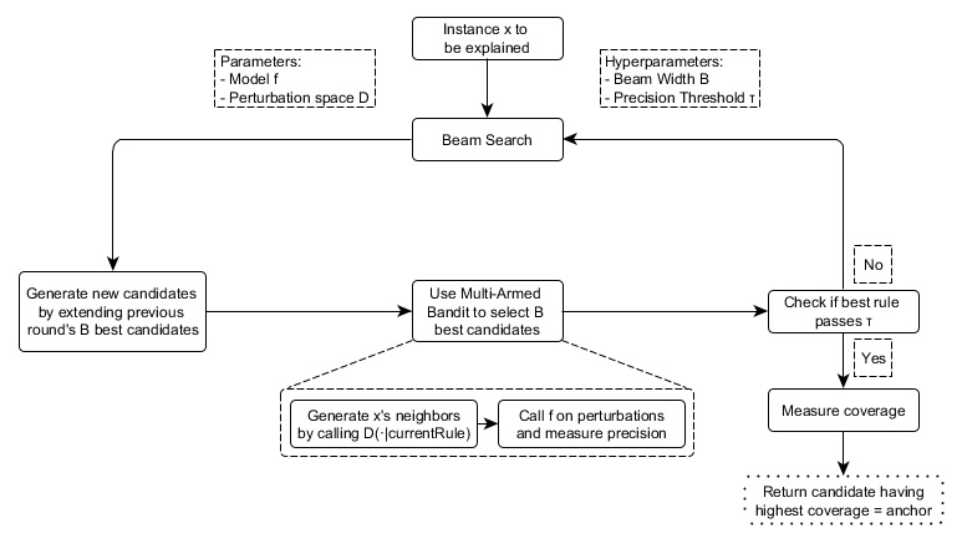
\includegraphics[scale=0.45]{pic/MA-Bilder/Literaturrecherche/Anchors_Finden.PNG}
%    \caption{Prozess zum Finden von Anchros, entnommen aus: \cite{molnar2022}}
%    \label{Fig:Anchors_Finden}
%\end{figure}

\textbf{Vor- und Nachteile}
Anchors sind einfach zu verstehen und werden dann angewendet, wenn alle Bedingungen der Regel erfüllt sind und weisen hierdurch eine hohe Genauigkeit auf \cite{ribeiro2018anchors}. Daneben können auch genaue Erklärungen entstehen, selbst wenn die lokale Nachbarschaft komplex ist. 
Anchors können sehr generell, aber gleichzeitig auch sehr spezifisch werden, was für Nutzer verwirrend sein könnte. Weiter müssen viele Modellaufrufe stattfinden, was zur Lasten der Performance geht. Weiter existiert bei der Bildklassifikation ein konzeptuelles Problem, da nicht klar ist, wie Abdeckung hier genau zu definieren ist \cite{molnar2022}.

\subsubsection{Kontrafaktische Erklärungen}
Kontrafaktische Erklärungen (engl. Counterfactual Explanations) beschreiben kausale Zusammenhänge in der Form \enquote{Wäre Merkmal A ein anderes gewesen, dann wäre auch die Vorhersage eine andere gewesen} \cite{molnar2022}. Sie bringen also Gegenargumente (engl. Counter Facts) für eine Vorhersage.

\subsubsection{Konzept}
Bisher beschriebene XAI-Methoden stellen heraus, inwiefern sich Merkmale auf eine Vorhersage auswirken. Kontrafaktische Erklärungen hingegen, beantworten die Frage, welche Änderungen an einer Eingabe vorgenommen werden müssen, um eine andere Vorhersage zu erhalten \cite{Nandi.2022}. Theoretisch wäre es zur Identifikation von kontrafaktischen Erklärungen möglich, zufällig Änderungen an der Eingabe vorzunehmen und zu beobachten, wie sich dies auf die Vorhersage auswirken würde. Zum einen ist dieses Vorgehen sehr rechenaufwendig, zum anderen hätte dies nach \textcite{molnar2022} keinen Mehrwert für Nutzer. Kontrafaktische Erklärungen lassen sich eher als eine Erklärung definieren, welche die kleinste Veränderung an der Eingabe wiedergeben, sodass sich die Vorhersage ändert. Es kann eher wünschenswert sein, dass eine kontrafaktischen Erklärung eine solche Vorhersagenerklärung ist, welche die kleinste Veränderung in den Merkmalswerten wiedergibt, was zu einer Änderungen in der Vorhersage führt. Eine Herausforderung, die diese Erklärungen meistern müssen, basiert auf dem sogenannten Rashomon-Effekt. Rashomon ist ein Film, in dem Akteure eine Geschichte aus unterschiedlichen Perspektiven erzählen. Jede einzelne Geschichte ist in sich schlüssig, jedoch widersprechen sie sich untereinander. Dieses Phänomen kann auch bei kontrafaktischen Erklärungen auftreten. So könnte eine Erlkärung verlangen den Wert $x_1$ zu ändern, während eine andere vorschlägt Merkmal $x_2$ zu modifizieren, es können also mehrere gültige kontrafaktische Erklärungen existieren. Es Um Anforderungen an die kontrafaktischen Erklärungen zu definieren ist es wichtig, dass Nutzer definieren, was genau eine relevante Veränderung in der Vorhersage einer Instanz ist (z.B. Genauigkeit oder andere Klasse). 
%Jedoch ist es nicht immer möglich, eine kontrafaktische Erklärung zu erstellen, welche den Nutzerwünschen gut entspricht. Als Beispiel sei hier genannt, dass es eine Klassifikation mit nur zwei Klassen gibt, die jedoch unausgeglichen verteilt sind. So liegen in der einen Klasse sehr viele und in der anderen sehr wenig Datenpunkte. So würde sich die Vorhersage zur weniger repräsentativen Klasse nur sehr schlecht ändern lassen (oder man müsste sehr viele Merkmale ändern). Hier sollte sich ein Nutzer dann dazu entscheiden, nicht die Klasse selbst, sondern die Genauigkeit der Vorhersage ändern zu wollen.
Daneben ist es in der Realität sinnvoll, solche Erklärungen zu geneieren, die ungefähr dem Original entsprechen. Bei einen Algorithmus, welcher bspw. die Preise für eine Wohnung vorhersagt, sollte die Quadratmeter-Zahl der Wohnung nicht negativ werden \cite{molnar2022}.

\textbf{Formale Grundlagen}
Für eine zu erklärende Instanz $x$ muss ein Kontrafakt $x'$ gefunden werden \cite{kamath2021explainable}. Für dieses $x'$ sollte das zugrundeliegende Modell $f$ die eine andere Vorhersage als für $x$ ausgeben, hier mit $y'$ notiert. Wie vorangegangen beschrieben, besteht weiter das Ziel, dass sich das Kontrafakt nicht besonders von der zu betrachtenden Instanz unterscheidet (hier durch $d$ angegeben). Dies lässt sich formal in folgendem Optimierungsproblem $L$ beschreiben\cite{kamath2021explainable}:
\begin{equation}
    \underset{x'}{min} \: L(x'|x) = (f(x')-y')^2 + \lambda d(x, x')
\end{equation}
$\lambda$ bestimmt das Verhältnis von $(f(x')-y')^2$ und der Distanzfunktion $d$. Für einen großes $\lambda$ wird ein Kontrafakt erstellt, welches sich in den Merkmalswerten von $x$ wenig unterscheidet. Für einen kleinen Wert werden solche Kontrafakte erstellt, die sich sehr nahe an der gewünschten Ausgabe $y'$ befinden. Das Kontrafakt $x'$ und dessen Merkmalswerte können nun genutzt werden, um mit Bezug auf die ursprüngliche Instanz eine Wenn-Dann-Regel aufzustellen, die beschreibt, welche Werte für eine andere Vorhersage geändert werden müsste.


%Für das Generieren dieser Erklärungen existieren unterschiedliche Möglichkeiten. Eine wurde von \textcite{wachter2017counterfactual} vorgestellt. Hier sind $w$ die Gewichte, $f$ ist der ML-Algorithmus, $yi$ ist die Zielvariable, $xi$ ist ein Datenpunkt. Gesucht ist nun ein Kontrafakt ($x'$), welches sich in der Nähe von $xi$ befindet, aber $fw(x)$ soll der von den Nutzern definierten Zielvariable $yi$ entsprechen. Nach \textcite{wachter2017counterfactual} ließe sich dies realisieren, indem folgende Gleichung minimiert wird, während $w$ nicht verändert wird: 
%\begin{equation}
%    arg \: \underset{x'}{min} \: \underset{\lambda}{max} \: \lambda (f_{w}(x') - y')^{2} + d(x_{i}, x')
%\end{equation}

%$d$ ist hier eine Funktion, welche berechnet, wie weit das Kontrafakt vom ursprünglichen Punkt $x$ entfernt ist. In Realität wird $\lambda$ maximiert, indem iterativ $x'$ gefunden wird und $\lambda$ erhöht wird \cite{wachter2017counterfactual}. Nach \cite{wachter2017counterfactual} kann für dieses Problem jeder Optimizer verwendet werden, 

\textbf{Anwendung}
Für kontrafaktische Ekärungen bestehen sowohl modell-agnostische (\cite{dhurandhar2019model, guidotti2018local}) als auch modellspezifische Ansätze (\textcite{wachter2017counterfactual, mothilal2020explaining}), welche sich z.B. die Gewichte von neuronalen Netzen zu Nutze machen. Die DICE-Bibliothek von Microsoft bietet Möglichkeiten zur Generierung von kontrafaktischen Erklärungen an \footnote{https://www.microsoft.com/en-us/research/project/dice/}. Beim Benutzen dieser Biblothek kann angegeben werden, wie viele kontrafaktische Erklärungen produziert werden soll.

\textbf{Vor- und Nachteile}
Ein Vorteil, welchen kontrafaktische Erklärungen gegenüber anderen Methoden wie z.B. LIME besitzen, ist ihre Genauigkeit. Sie stellen relativ klar heraus, welche Merkmale geändert werden müssen. LIME z.B. kann keine Aussagen über den genauen Wert geben, da diese nur lokale Genauigkeit besitzen, wie in Abbilung \ref{Fig:Lime-Funktionsweise} gezeigt. Daneben sind sie für Menschen gut verständlich \cite{molnar2022}. Ein Nachteil dieser XAI-Methode besteht in dem grundsätzlichen Rashomon-Effekt, der es erschwert, die richtige Erklärung auszuwählen \cite{kamath2021explainable}. Im Zweifel sollten den Nutzer daher eine größere Zahl vieler verschiedener Erklärungen präsentiert werden \cite{molnar2022}. Daneben haben einige Methoden, z.B. die von \cite{wachter2017counterfactual} zum Finden der Kontrafakte, dass Problem, nicht nur solche Kontrafakte zu finden, welche wenig Merkmale abändern. Des Weiteren werden auch unrealistische Merkmale miteinbezogen \cite{molnar2022}
%Dies wird von einer anderen Methode jedoch erfüllt (\cite{dandl2020multi}).

